
\documentclass[11pt]{article}

% ================= _preamble =================
\usepackage[utf8]{inputenc}

\usepackage[spanish, es-tabla, es-noshorthands]{babel}
\usepackage{amsmath}
\usepackage{amsfonts}
\usepackage{amssymb}
\usepackage{csquotes}
\usepackage[left=20mm, top=20mm, bottom=20mm, right=20mm]{geometry}
\usepackage{sectsty}
\usepackage[T1]{fontenc}
\usepackage{graphicx}
\usepackage{fancyhdr}
\usepackage{float}
\usepackage{nameref}
\usepackage{url}
\usepackage{enumerate}
\usepackage{array} % required for text wrapping in tables
\usepackage{tikz}
\usetikzlibrary{arrows.meta, positioning, fit}

% \addto\captionsspanish{% Replace "english" with the language you use
%   \renewcommand{\contentsname}%
%     {Contenido}%
% }

\setlength{\headheight}{15pt}

\newcommand\blankpage{%
    \null
    \thispagestyle{empty}%
    \addtocounter{page}{-1}%
    \newpage}
    
% \usepackage[usefilenames,% Important for XeLaTeX
%   RMstyle={Medium,Semibold},
%   SSstyle={Medium,Semibold},
%   TTstyle={Medium,Semibold},
%   DefaultFeatures={Ligatures=Common}]{plex-otf} %
% \renewcommand*\familydefault{\sfdefault}

\renewcommand{\headrulewidth}{0pt}
\renewcommand{\footrulewidth}{0.7pt}

\makeatletter

\newcommand\frontmatter{%
    \pagestyle{plain}
    \allsectionsfont{\normalfont\rmfamily\bfseries}
    \cleardoublepage
  %\@mainmatterfalse
  \pagenumbering{roman}}

\newcommand\mainmatter{%
    \allsectionsfont{\usefont{T1}{lmss}{b}{m}}
    \cleardoublepage
 % \@mainmattertrue
  \pagenumbering{arabic}
  \pagestyle{fancy}
  \rhead[]{Diseño y desarrollo de un juguete STEAM mediante energy harvesting
para la enseñanza de conceptos relacionados con la transformación y el
aprovechamiento de la energía}
  \lhead[]{}
  \lfoot[]{}
  \rfoot[]{}
  \renewcommand{\headrulewidth}{0.7pt}
  \renewcommand{\footrulewidth}{0pt}}
\newcommand\backmatter{%
    \newpage
    \pagestyle{plain}
    \allsectionsfont{\normalfont\rmfamily\bfseries}
    \setcounter{section}{0}
    \renewcommand{\thesection}{\Alph{section}}
   }

\makeatother

\newcommand\blfootnote[1]{%
  \begingroup
  \renewcommand\thefootnote{}\footnote{#1}%
  \addtocounter{footnote}{-1}%
  \endgroup
}

\usepackage[backend=biber, style=ieee]{biblatex}
\addbibresource{bibliography.bib}


\usepackage[
    pdfauthor={Nombre del Autor},
    pdftitle={Título del Documento},
    pdfsubject={Temática o Campo del Conocimiento},
    pdfkeywords={Palabras Clave},
    pdfproducer={Latex},
    pdfcreator={pdflatex},
    hidelinks
]{hyperref}

\begin{document}

% Portada
% ================= _cover =================
\pagestyle{empty}
%\afterpage{\blankpage}
\begin{center}

\Large
\hrule
\vspace{4mm}
\textbf{Diseño y desarrollo de un juguete steam mediante \textit{energy harvesting} para la enseñanza de conceptos relacionados con la transformación y el aprovechamiento de la energía.}
\vspace{4mm}
\hrule
\large
\vfill
Autores\\
Alejandro Llerena Pinzón \\
Daniel Francisco Peña Blanco
\vfill
Director\\
Arturo Fajardo Jaimes
\vfill
Cliente\\
Fundación Colegio Emilio Valenzuela
\vfill
\begin{figure}[h]
\centering

\includegraphics[width=1.5in]{LogoPUJ.png}
\label{escudo}
\end{figure}

Facultad de Ingeniería\\
\textit{Ingeniería Mecatrónica}\\
\vspace{4mm}
Bogotá - Colombia, 10 de noviembre de 2026
\end{center}
\newpage


% Tabla de contenido
% ================= _table_of_contents =================
\addtocontents{toc}{\hfill \textbf{Página} \par}
\tableofcontents
\newpage
%\listoffigures
%\newpage
%\listoftables
%\newpage


% Resumen (opcional)
% \input{source/resumen}

% Contenido principal
% ================= introduccion =================
\section{Introducción}

La educación STEAM (Ciencia, Tecnología, Ingeniería, Artes y Matemáticas) busca integrar diferentes áreas del conocimiento mediante experiencias prácticas que permitan a los estudiantes relacionar los conceptos científicos con situaciones de la vida cotidiana. Dentro de este enfoque, la energía constituye un concepto fundamental debido a su relación con fenómenos y aplicaciones presentes en diferentes áreas de la ciencia y la tecnología. Sin embargo, su parte teórica genera dificultades de comprensión en los estudiantes, quienes pueden presentar concepciones alternativas relacionadas con qué es la energía, sus fuentes y sus procesos de transformación \cite{Domenech2018}.En Colombia, esta dificultad se refleja en los resultados de las pruebas Saber 11: en la aplicación nacional de 2024, el 68.28\% de los estudiantes se ubicó en los niveles de desempeño insuficiente o mínimo en el área de Ciencias Naturales, cifra que, si bien representa una reducción frente al 76.6\% registrado en 2021, evidencia que la mayoría de los estudiantes del país continúa sin alcanzar un dominio satisfactorio de los conceptos evaluados en esta área.\cite{ICFES2024}

Esta dificultad evidencia la necesidad de implementar estrategias educativas que permitan abordar el tema de una forma más interactiva. Siendo así, el enfoque STEM ofrece una alternativa al aprendizaje exclusivamente teórico. Un estudio realizado con 143 estudiantes de noveno grado encontró que una intervención basada en STEM y el modelo 5E, aplicada durante siete sesiones para abordar conceptos de energía y conversión de energía solar, produjo mejoras significativas en el rendimiento académico y la creatividad de los estudiantes \cite{Shahbazloo2023}. Esto demuestra la importancia de crear experiencias en las que el estudiante pueda explorar, experimentar y aplicar los conceptos aprendidos.

Dentro de las estrategias utilizadas para fortalecer este tipo de aprendizaje se encuentran los juguetes STEM. Una revisión sistemática que analizó 2352 artículos y seleccionó 32 estudios mostró que estos recursos pueden favorecer habilidades como la resolución de problemas, el pensamiento crítico, la creatividad y la colaboración, especialmente cuando se acompañan de actividades experimentales y aprendizaje mediante prueba y error \cite{Pandey2025}. En Colombia, un estudio con estudiantes de básica primaria evaluó el uso de juguetes alimentados con energía solar como estrategia para la enseñanza de las ciencias naturales, encontrando resultados favorables en el proceso de enseñanza-aprendizaje \cite{MendozaMendoza2025}. Sin embargo, esta y otras experiencias similares se han limitado a la alimentación directa de los dispositivos mediante paneles solares, sin incorporar sistemas de conversión, acondicionamiento y almacenamiento de energía, ni estar dirigidas a estudiantes de bachillerato. En una línea complementaria, otra revisión sistemática analizó 584 artículos sobre \textit{serious games} en educación STEM y seleccionó 37 estudios, encontrando efectos positivos sobre la adquisición y aplicación de conocimientos, así como la motivación y participación de los estudiantes \cite{Tene2025}. Resultados como estos respaldan el uso de recursos educativos que combinen el aprendizaje con la interacción.

Desde el punto de vista tecnológico, el \textit{Energy Harvesting} permite aprovechar energía disponible en el entorno y transformarla en energía eléctrica utilizable para alimentar dispositivos electrónicos. Fernández Ramos desarrolló experimentalmente un sistema de \textit{Piezoelectric Energy Harvesting} en el que las vibraciones mecánicas eran convertidas en energía eléctrica mediante un transductor piezoeléctrico y un circuito de acondicionamiento, logrando utilizar la energía obtenida para alimentar un dispositivo electrónico \cite{FernandezRamos2017}. Por ello, este tipo de tecnología muestra una oportunidad para trasladar un fenómeno físico a una experiencia educativa observable. No obstante, pese al potencial demostrado del \textit{energy harvesting} en aplicaciones técnicas y a la evidencia sobre los beneficios de los juguetes STEM en la enseñanza de las ciencias, no se identificaron desarrollos —ni en el contexto colombiano ni en la literatura revisada— que integren un sistema de \textit{energy harvesting} solar y piezoeléctrico dentro de un juguete STEAM orientado a la enseñanza de la transformación energética en estudiantes de bachillerato. Este vacío se acentúa si se considera que las experiencias colombianas disponibles hasta ahora se han limitado a niveles de básica primaria, dejando sin explorar el potencial de este tipo de recursos en etapas educativas donde los conceptos de conversión energética adquieren mayor complejidad curricular.

En consecuencia, surge la necesidad de desarrollar un recurso educativo interactivo que integre la experimentación con conceptos relacionados con la energía y sus procesos de transformación. Por ello, este proyecto propone el diseño y desarrollo de un juguete STEAM que incorpore un sistema de \textit{Energy Harvesting} basado en un harvester solar y uno piezoeléctrico, cuya energía será acondicionada y almacenada en una batería para alimentar los diferentes componentes del juguete. El sistema estará orientado a generar una experiencia educativa para estudiantes de bachillerato, mediante actividades y guías que permitan abordar de manera práctica conceptos relacionados con la transformación y el aprovechamiento de la energía.

% ================= problema =================
\newpage
\section{Descripción del Problema}
En la educación media, comprender la energía representa un desafío porque exige relacionar sus fuentes, formas, transferencias, transformaciones y conservación. Goldring y Osborne encontraron que al menos el 50\% de 75 estudiantes tenía dificultades para comprender conceptos básicos de energía y aplicarlos a situaciones cotidianas \cite{goldring1994}. Bächtold y Munier también identificaron confusiones entre energía, fuerza, calor y potencia. En su estudio con estudiantes de grado 11, después de una intervención didáctica, las respuestas inadecuadas sobre transformaciones energéticas disminuyeron del 58\% al 41\%, pero las explicaciones completas solo aumentaron del 2\% al 14\% \cite{bachtold2019}. Esto evidencia que no basta con resolver ejercicios: se requiere comprender los fenómenos energéticos de manera integrada.

Esta dificultad puede agravarse cuando los contenidos se presentan principalmente de forma teórica y con pocas oportunidades de experimentación. Buldur \textit{et al.} advierten esta limitación en la enseñanza formal de las energías renovables y reportan que un proyecto al aire libre con 60 estudiantes mejoró significativamente el conocimiento técnico y las perspectivas de uso futuro, aunque no todos los factores evaluados cambiaron significativamente \cite{buldur2020}. En concordancia, Whitelegg y Parry destacan la importancia de relacionar la física con situaciones de la vida real \cite{whitelegg1999}. Los resultados de experiencias prácticas también respaldan este enfoque: Rachniyom \textit{et al.} encontraron que, tras experimentos sobre la transformación de energía potencial en cinética, el promedio de 30 estudiantes de grado 10 pasó del 34,33\% al 93,33\% entre la prueba inicial y la final \cite{rachniyom2017}. Asimismo, Kanapathy y Azhari observaron una mejora estadísticamente significativa después de actividades prácticas STEM con 47 estudiantes \cite{kanapathy2024}. Por su parte, Hsiao \textit{et al.} encontraron que, frente al aprendizaje basado en proyectos (PBL) por sí solo, la incorporación de un modelo de interacción cognitivo-afectiva en una actividad de construcción de un bote eléctrico mejoró el conocimiento STEAM, la creatividad y el desempeño práctico de 366 estudiantes \cite{hsiao2022}.

En Colombia, Cárdenas \textit{et al.} desarrollaron el kit ``Caja Solar'', que permite experimentar con un panel fotovoltaico, controlador de carga, baterías y medición de variables eléctricas. Sin embargo, su alcance se concentra en la enseñanza de sistemas fotovoltaicos y la evaluación reportada recoge la percepción de 17 participantes \cite{cardenas2024}. En los antecedentes revisados se encuentran experimentos sobre transformaciones mecánicas, actividades STEAM y herramientas para aprender energía solar, pero no se aborda conjuntamente la integración de estos elementos en un juguete interactivo que combine captación solar y piezoeléctrica, acondicionamiento, gestión y almacenamiento energético, y sistemas de control y actuación.

Si esta necesidad no se atiende, pueden persistir las dificultades para explicar cómo se genera, transforma, almacena y utiliza la energía en aplicaciones reales, limitando la conexión entre el conocimiento científico y su aprovechamiento tecnológico. Por tanto, el problema que aborda este trabajo es la brecha entre la enseñanza conceptual de las transformaciones energéticas y la disponibilidad de una experiencia didáctica interactiva que permita experimentarlas de forma integrada. Se requiere diseñar y desarrollar un juguete STEAM con sistemas de \textit{energy harvesting} solar y piezoeléctrico, acondicionamiento y gestión para almacenar la energía generada y contribuir a la autosostenibilidad del prototipo, junto con sistemas de control, actuación e interacción. Además, deberán verificarse la capacidad de generación bajo condiciones definidas, la integración y el funcionamiento de los subsistemas, y evaluarse con estudiantes de bachillerato su aporte a la comprensión de conceptos relacionados con la transformación y el aprovechamiento de la energía.

% ================= objetivos =================
\newpage
\section{Objetivos}
\subsection{Objetivo General}
\textit{Diseñar y desarrollar un juguete STEAM mediante el uso de sistemas de \textit{Energy Harvesting} que contribuyan a aumentar su autosostenibilidad energética, orientado a la enseñanza de conceptos relacionados con la transformación y el aprovechamiento de la energía.}


\subsection{Objetivos Específicos}

\begin{itemize}
    \item Diseñar un sistema de \textit{Energy Harvesting} compuesto por un harvester solar y uno piezoeléctrico, junto con el sistema de acondicionamiento y gestión energética para el almacenamiento de la energía generada, determinando su capacidad de generación bajo condiciones de operación definidas.
    
    \item Diseñar y desarrollar un prototipo funcional de juguete STEAM que integre el sistema de control, los actuadores y la interfaz de interacción, alimentados mediante un sistema de almacenamiento energético de acuerdo con los requerimientos funcionales y energéticos establecidos.
    
    \item Integrar el sistema de \textit{Energy Harvesting} y almacenamiento energético con el prototipo de juguete STEAM, verificando el funcionamiento conjunto de los subsistemas de generación, almacenamiento, control y actuación.

    \item Evaluar una experiencia educativa con estudiantes de bachillerato mediante el uso del prototipo de juguete STEAM, aplicando un instrumento de evaluación orientado a analizar la comprensión de conceptos relacionados con la transformación y el aprovechamiento de la energía.
     
\end{itemize}

% ================= requerimientos =================
\newpage
\section{Requerimientos}


\subsubsection{Requerimientos Funcionales}
\begin{itemize}
  \item \textbf{Tracción:} El robot debe avanzar, retroceder, girar y rotar sobre su propio eje mediante tracción diferencial de dos motores.
  \item \textbf{Control de Velocidad y Distancia:} Debe usar la lectura de los encoders para regular la velocidad de cada rueda y estimar la distancia recorrida (odometría).
  \item \textbf{Modos de Operación:} Debe ofrecer dos modos: control remoto en tiempo real y ejecución de secuencias programadas por el estudiante.
  \item \textbf{Detección de Obstáculos} Debe incorporar al menos un sensor de distancia (ultrasónico o infrarrojo) que detenga el robot ante un obstáculo cercano y que pueda usarse dentro de los programas.
  \item \textbf{Indicadores:} Debe mostrar, mediante LEDs o una pantalla pequeña, el nivel de batería, el estado de conexión, el modo activo y si está recibiendo energía cosechada.
\end{itemize}
 
\subsubsection{Requerimientos de Calidad}
\begin{itemize}
  \item \textbf{Autonomía:} Al menos 60 minutos de uso continuo con batería completa (una sesión de clase con margen).
  \item \textbf{Robustez:} Debe resistir el uso repetido en aula y caídas desde la altura de un pupitre (aprox. 0,75\,m) sin perder funcionalidad.
  \item \textbf{Tamaño y Peso:} Compacto y manipulable por un estudiante con una mano; peso objetivo inferior a 1\,kg.
  \item \textbf{Precisión de Movimiento}  Error de distancia inferior al 10\,\% en trayectos rectos de 1\,m sobre superficie plana.
\end{itemize}
 
\subsubsection{Requerimientos de Implementación}
\begin{itemize}
  \item \textbf{Microcontrolador:} ESP32-C3 Super Mini, encargado del control de motores, la lectura de sensores y la comunicación inalámbrica.
  \item \textbf{Actuadores:} Dos motorreductores de 6\,V con encoder y un driver de motores (puente H) dimensionado para su corriente de arranque.
  \item \textbf{Chasis:} Plataforma 2WD tipo DFRobot Tortuga (ROB0005) o equivalente, con puntos de montaje para añadir módulos.
  \item \textbf{Diseño Abierto y Modular}  Los componentes internos deben ser visibles (carcasa transparente o abierta) y las conexiones deben estar etiquetadas para que el estudiante identifique cada subsistema.
\end{itemize}
 

\subsection{Requerimientos del Sistema de Energía (Energy Harvesting)}
 
\subsubsection{Requerimientos Funcionales}
\begin{itemize}
  \item \textbf{Fuente Principal de Recolección:} Panel solar fotovoltaico que recargue la batería del robot.
  \item \textbf{Fuente Secundaria Demostrativa:} Módulo piezoeléctrico orientado a demostrar la conversión mecánica-eléctrica; no se espera que sostenga la operación de los motores.
  \item \textbf{Gestión de Energía:} Un módulo basado en el controlador CN3791 debe
gestionar la carga de la batería de una celda y realizar el seguimiento del
punto de máxima potencia (MPPT) de la fuente fotovoltaica. La fuente
piezoeléctrica se considera secundaria y demostrativa, y no se asumirá que el
MPPT del CN3791 realiza su seguimiento \cite{consonance_cn3791}.
  \item \textbf{Arquitectura de Potencia Separada}  La etapa de recolección solo debe cargar la batería y alimentar la electrónica de bajo consumo; los motores deben alimentarse desde la batería mediante una etapa de potencia dedicada.
  \item \textbf{Medición de Energía}  El sistema debe medir el voltaje de la batería y, de ser posible, la corriente de carga, y enviar estos datos a la aplicación.
\end{itemize}
 
\subsubsection{Requerimientos de Calidad}
\begin{itemize}
  \item \textbf{Tiempo de Recarga:} Debe caracterizarse el tiempo de recarga bajo luz solar directa y bajo iluminación de aula; meta preliminar: recuperar el 50\,\% de la batería en una jornada escolar con luz solar.
  \item \textbf{Bajo Consumo en Reposo:} En modo reposo (\textit{deep sleep}) el consumo total debe ser inferior a 1\,mA para no agotar la batería entre clases.
  \item \textbf{Uso Durante la Carga} El robot debe poder operar mientras recibe energía, sin daño para la batería ni para el circuito de gestión.
\end{itemize}
 
\subsubsection{Requerimientos de Seguridad Eléctrica }
\begin{itemize}
  \item \textbf{Protección de Batería:} Protección contra sobrecarga, descarga profunda y cortocircuito (BMS o módulo de protección).
  \item \textbf{Aislamiento:} La batería y las conexiones de potencia no deben ser accesibles sin herramienta.
  \item \textbf{Interruptor General:} Interruptor físico de encendido/apagado visible y de fácil acceso.
\end{itemize}
 

\subsection{Requerimientos de Comunicación y Control}
 
\subsubsection{Requerimientos Funcionales}
\begin{itemize}
  \item \textbf{Conectividad Inalámbrica:} Control desde celular o computador mediante Bluetooth Low Energy o Wi-Fi del ESP32-C3.
  \item \textbf{Control Alternativo:} Compatibilidad con un control físico independiente para usuarios sin dispositivo propio.
  \item \textbf{Parada Segura (\textit{Failsafe})} : Si se pierde la conexión por más de 500\,ms, los motores deben detenerse automáticamente.
\end{itemize}
 
\subsubsection{Requerimientos de Calidad}
\begin{itemize}
  \item \textbf{Latencia:} Tiempo entre la orden y la respuesta del robot inferior a 200\,ms.
  \item \textbf{Alcance:} Al menos 10\,m en interiores.
  \item \textbf{Operación en Aula con Varios Robots} : Varios robots deben operar en el mismo salón sin interferencias, con emparejamiento único entre cada robot y su controlador.
\end{itemize}
 

\subsection{Requerimientos de la Aplicación (Control y Programación)}
 
\subsubsection{Requerimientos Funcionales}
\begin{itemize}
  \item \textbf{Interfaz de Control Remoto:} Joystick o botones direccionales y control de velocidad.
  \item \textbf{Programación por Niveles} : Programación por bloques para principiantes y opción de código (p.\,ej. MicroPython) para estudiantes avanzados.
  \item \textbf{Panel de Energía} : Visualización en tiempo real de la energía recolectada frente a la consumida, con histórico de la sesión.
  \item \textbf{Retos Guiados:} Actividades predefinidas por nivel de dificultad dentro de la aplicación.
\end{itemize}
 
\subsubsection{Requerimientos de Calidad}
\begin{itemize}
  \item \textbf{Compatibilidad:} Funcionamiento en Android, iOS y computadores, preferiblemente sin instalación (aplicación web).
  \item \textbf{Facilidad de Uso} : Un estudiante sin experiencia previa debe lograr mover el robot en menos de 10 minutos (métrica a validar en pruebas con usuarios).
\end{itemize}
 
\subsubsection{Requerimientos de Seguridad y Privacidad}
\begin{itemize}
  \item \textbf{Minimización de Datos} : La aplicación no debe exigir cuentas ni recolectar datos personales de los estudiantes, que en su mayoría son menores de edad.
  \item \textbf{Perfil Docente:} Opción de perfil para el docente que permita gestionar retos y robots del aula.
\end{itemize}
 

\subsection{Requerimientos Pedagógicos (STEAM) }
\begin{itemize}
  \item \textbf{Cobertura de las Áreas STEAM:} Cada área debe tener al menos una actividad asociada: Ciencia (conversión y almacenamiento de energía), Tecnología (control inalámbrico), Ingeniería (diseño y ajuste del sistema), Arte (personalización de la carcasa) y Matemáticas (odometría, velocidad, cálculo de energía).
  \item \textbf{Alineación Curricular:} Las actividades deben relacionarse con las orientaciones del Ministerio de Educación Nacional para educación en tecnología (Guía 30) y con los estándares de ciencias naturales para grados noveno a once.
  \item \textbf{Material de Apoyo:} Guía docente y fichas de actividades con objetivos de aprendizaje y forma de evaluación.
\end{itemize}
 

\subsection{Requerimientos de Seguridad del Usuario y Normativos }
\begin{itemize}
  \item \textbf{Seguridad Física:} Sin bordes cortantes ni puntos de atrapamiento en ruedas y engranajes accesibles.
  \item \textbf{Temperatura Superficial:} Ninguna superficie accesible debe alcanzar temperaturas que generen riesgo de quemadura durante la operación o la carga.
  \item \textbf{Normas de Referencia:} El diseño debe tomar como referencia ISO 8124 (seguridad de juguetes) e IEC 62115 (seguridad de juguetes eléctricos).
\end{itemize}

\subsection{Requerimientos de Sostenibilidad y Viabilidad }
\begin{itemize}
  \item \textbf{Reparabilidad:} Batería, motores y sensores reemplazables con herramientas básicas.
  \item \textbf{Componentes Comerciales:} Uso de componentes disponibles en el mercado colombiano.
  \item \textbf{Costo Objetivo:} Costo de materiales por unidad definido y comparado con kits educativos de robótica disponibles en el mercado.
\end{itemize}



% ================= estadodelarte =================
\newpage
\section{Estado del Arte}
 
\subsection{Plataformas robóticas educativas de bajo costo}
 
La robótica educativa ha avanzado hacia plataformas abiertas y económicas que
reemplazan los kits comerciales costosos. Piljek et al.~\cite{piljek2023mobile} usaron un
robot de tracción diferencial, con piezas de fabricación propia y un microcontrolador de
bajo costo, como base para actividades de aprendizaje con estudiantes de colegio. En el
mercado colombiano, esta misma arquitectura se encuentra en chasis listos para ensamblar,
como la plataforma Tortuga 2WD (ROB0005)~\cite{sigma2026rob0005} y el chasis MiniQ 2WD
(ROB0049)~\cite{sigma2026rob0049} de DFRobot, que incluyen dos motorreductores de 6\,V y
rueda loca, y cuyo precio los hace viables para un proyecto replicable en colegios.
 
Estos trabajos validan la tracción diferencial con dos
motorreductores como una configuración sencilla, económica y suficiente para que el
robot avance, retroceda, gire y rote sobre su eje. Esto permite que el proyecto concentre
su aporte en el sistema energético y en la experiencia de aprendizaje, y no en el
desarrollo de una plataforma mecánica nueva. Los chasis Tortuga y MiniQ son la base
física del prototipo: ya traen los dos motorreductores y el espacio para montar el
ESP32-C3, la batería y los elementos de captación, y se consiguen en el país. Sin
embargo, ninguno de estos trabajos o productos aborda la fuente de energía del robot como
contenido de enseñanza.
 
\subsection{El robot como objeto de estudio de la energía}
 
Gabbanelli y Szigety~\cite{gabbanelli2023robot} mostraron que un robot de bajo costo con
dos motorreductores puede convertirse en un objeto de estudio en la clase de física:
sus estudiantes de bachillerato midieron la potencia mecánica y eléctrica del robot y
discutieron por qué el balance energético no cerraba. Por su parte, Mustafa et
al.~\cite{mustafa2026solar} y Che Rozi y Jafferi~\cite{cherozi2024solar} evidenciaron
que, en robots móviles con paneles solares, el consumo de los motores supera lo que
entrega un panel pequeño, por lo que la batería sigue siendo indispensable.
 
Gabbanelli y Szigety confirman que medir la energía de un
robot permite a los estudiantes trabajar conceptos de transformación y disipación con
datos propios, lo que respalda el enfoque pedagógico de la propuesta. Los estudios de
robots solares justifican una decisión central del diseño: usar la captación como apoyo
a la batería de litio y no como fuente única. El vacío que dejan estos trabajos es que
ninguno integra la captación de energía en un robot con propósito educativo.
 
\subsection{La captación de energía como actividad educativa}
 
La captación de energía ya se ha llevado al aula, aunque en montajes estáticos.
Mendoza-Mendoza y Vásquez-Benítez~\cite{mendoza2025juguetes} reportaron resultados
favorables con juguetes solares en Colombia, y Heeter et al.~\cite{heeter2016maker}
encontraron mejoras en el aprendizaje de estudiantes de bachillerato tras actividades con
elementos piezoeléctricos evaluadas antes y después. Arvanitou et
al.~\cite{arvanitou2025piezo} propusieron una secuencia para grado once basada en el
modelo predecir-observar-explicar para estudiar la captación piezoeléctrica.
 
Estos trabajos muestran que tanto la energía solar como la
piezoeléctrica son contenidos accesibles y motivadores para estudiantes de colegio, y
ofrecen estrategias que la propuesta puede adoptar: la evaluación antes y después de la
intervención y la secuencia predecir-observar-explicar. Su limitación es que trabajan
cada fuente por separado y en objetos que no se mueven, mientras que esta propuesta las
integra en un juguete móvil.
 
\subsection{Sistemas híbridos de captación solar y piezoeléctrica}
 
Diversos estudios han combinado ambas fuentes en un mismo sistema de almacenamiento.
Alfonso et al.~\cite{alfonso2021plant} y Baltazar et al.~\cite{baltazar2023turnstile}
integraron captación solar y piezoeléctrica con circuitos de gestión de energía para
cargar baterías, y en ambos casos la fuente piezoeléctrica aportó una fracción mínima
frente a la solar. La revisión de Sharma et al.~\cite{sharma2022tiles} confirma que la
energía piezoeléctrica es adecuada solo para cargas de muy baja potencia.
 
Estos trabajos demuestran que es viable combinar ambas
fuentes hacia una misma batería mediante un circuito integrado de gestión, como el
CN3791 que se evalúa en esta propuesta. También establecen una expectativa realista:
la fuente piezoeléctrica se incorpora por su valor demostrativo, para que los estudiantes
comparen cuánto aporta cada fuente, y no por su contribución energética. Ninguno de estos
sistemas tiene propósito educativo ni alimenta motores.
 
 
 




% ================= marco_teorico =================
\newpage
\section{Marco Teórico}

\subsection{Energy harvesting}
El \emph{energy harvesting} (recolección de energía) consiste en convertir
energía ambiental —luz, vibraciones, movimiento, gradientes térmicos— en
energía eléctrica utilizable por un dispositivo electrónico
\cite{sudevalayam2011}. Su principal ventaja es reducir la dependencia de
baterías desechables y extender la autonomía del sistema; su principal
limitación es que la potencia disponible es baja e intermitente, por lo que
en general no alimenta la carga de forma directa, sino que repone un elemento
de almacenamiento \cite{knight2008}.
 
Un sistema de recolección se compone de cuatro etapas (Fig.~\ref{fig:arq}):
(i) la fuente y su transductor, (ii) el acondicionamiento de potencia
(rectificación y conversión DC/DC), (iii) el almacenamiento (batería o
supercapacitor) y (iv) la carga \cite{sudevalayam2011}. La comparación de
densidades de potencia de distintas fuentes muestra que la solar en exteriores
supera en varios órdenes de magnitud a la de vibraciones, mientras que en
interiores ambas se vuelven comparables \cite{roundy2003}. Este resultado
justifica combinar dos fuentes complementarias: la solar, cuando hay luz
disponible, y la piezoeléctrica, que depende de la interacción del usuario con
el juguete.
 
\begin{figure}[htbp]
\centering
\begin{tikzpicture}[
  node distance=0.45cm and 0.5cm,
  box/.style={draw, rounded corners, align=center, font=\scriptsize,
              minimum height=0.8cm, text width=1.7cm},
  arr/.style={-{Stealth[length=2mm]}, thick}]
  \node[box] (sol) {Panel solar\\(DC)};
  \node[box, below=of sol] (piezo) {Piezoeléctrico\\(AC)};
  \node[box, right=of piezo] (rect) {Rectificador +\\capacitor};
  \node[box, right=of rect, yshift=0.62cm] (cn) {CN3781\\cargador\\buck CC/CV};
  \node[box, right=of cn] (bat) {Batería\\Li-ion\\1 celda};
  \node[box, right=of bat] (load) {Regulación +\\ESP32-C3 +\\motores};
  \draw[arr] (sol.east) -- (cn.west |- sol.east);
  \draw[arr] (piezo) -- (rect);
  \draw[arr] (rect.east) -- (cn.west |- rect.east);
  \draw[arr] (cn) -- (bat);
  \draw[arr] (bat) -- (load);
\end{tikzpicture}
\caption{Arquitectura de alimentación del juguete: dos fuentes de recolección,
acondicionamiento, carga de la batería y alimentación de la carga.}
\label{fig:arq}
\end{figure}
 
\subsection{Conversión fotovoltaica}
Una celda solar es una unión p-n en la que los fotones con energía superior a
la banda prohibida del semiconductor generan pares electrón-hueco que producen
una corriente continua. Su eficiencia tiene un límite teórico de alrededor del
30\,\% para una celda de unión simple con banda prohibida de 1{,}1~eV
\cite{shockley1961}, y en la práctica es menor. La potencia máxima entregada
se expresa como
\begin{equation}
  P_{\max} = FF \cdot V_{oc} \cdot I_{sc} = \eta \, G \, A ,
  \label{eq:pv}
\end{equation}
donde $FF$ es el factor de llenado, $V_{oc}$ y $I_{sc}$ son el voltaje de
circuito abierto y la corriente de cortocircuito, $\eta$ la eficiencia, $G$ la
irradiancia y $A$ el área. La ecuación~\eqref{eq:pv} explica por qué el
rendimiento del juguete dependerá fuertemente del lugar de uso (exterior o
interior) y del área de panel que se pueda integrar en su diseño.
 
\subsection{Conversión piezoeléctrica}
Los materiales piezoeléctricos (p.\,ej., cerámicas PZT o polímeros PVDF)
generan carga eléctrica cuando se deforman mecánicamente. En una aproximación
simple, la carga generada es proporcional a la fuerza aplicada, $Q = d_{33}F$,
y el voltaje en circuito abierto es $V = Q/C_p$, siendo $d_{33}$ el coeficiente
piezoeléctrico y $C_p$ la capacitancia del elemento \cite{priya2007}. A
diferencia del panel solar, la salida es alterna, de alto voltaje y baja
corriente, y la fuente presenta una impedancia interna elevada; por ello
requiere un rectificador y un capacitor de acumulación antes de entregar
energía a un convertidor DC/DC \cite{ottman2002}. Experiencias con
transductores accionados por movimiento humano, como los integrados en el
calzado, muestran potencias promedio del orden de milivatios
\cite{shenck2001}, lo que confirma que esta fuente es adecuada para
\emph{reponer} energía, no para alimentar motores de forma continua.
 
\subsection{Carga de la batería mediante el CN3791}

El CN3791 es un controlador conmutado PWM de topología reductora (\textit{buck})
para la carga de una batería de ion-litio de una celda desde una fuente
fotovoltaica. Implementa las etapas de precarga, corriente constante y tensión
constante. La tensión de regulación en la etapa de tensión constante es
\(4.2\,\mathrm{V}\pm 1\,\%\). La corriente de carga se establece mediante una
resistencia externa de sensado y puede alcanzar hasta \(4\,\mathrm{A}\), de
acuerdo con los límites del circuito y de los componentes externos
\cite{consonance_cn3791,consonance_cn3791_datasheet}.

El seguimiento del punto de máxima potencia se realiza mediante el método de
tensión constante. El pin MPPT se regula a un valor típico de
\(1.205\,\mathrm{V}\), mientras que un divisor resistivo establece el voltaje
de operación objetivo del panel:

\begin{equation}
V_{\mathrm{MPPT}} =
1.205\left(1+\frac{R_3}{R_4}\right).
\end{equation}

Por tanto, la selección de \(R_3\) y \(R_4\) debe corresponder al voltaje de
máxima potencia del panel que se integre. Este método está referido al panel
fotovoltaico; no debe presentarse como MPPT de la fuente piezoeléctrica
\cite{consonance_cn3791_datasheet}.

El CN3791 es el controlador integrado, no necesariamente una tarjeta lista
para conectar. Su circuito de aplicación requiere componentes externos,
entre ellos un MOSFET de canal P, un inductor, una resistencia de sensado y
capacitores. Si se emplea un módulo comercial, sus valores y prestaciones
deben tomarse de la documentación de esa tarjeta específica. El fabricante
especifica un rango de entrada de \(4.5\) a \(28\,\mathrm{V}\), frecuencia de
conmutación típica de \(300\,\mathrm{kHz}\) y carga de una batería por celda
a \(4.2\,\mathrm{V}\) \cite{consonance_cn3791_datasheet}. Al ser un cargador de entrada DC, la señal del
piezoeléctrico debe rectificarse y acumularse previamente
(Fig.~\ref{fig:arq}).
 
\subsection{Balance energético del sistema}
La viabilidad de la propuesta depende de comparar la energía recolectada con la
energía consumida por la carga —el microcontrolador ESP32-C3, su radio
inalámbrica y los dos motorreductores de la plataforma móvil
\cite{sigma2026rob0005}— durante un ciclo de uso:
\begin{equation}
  \underbrace{\textstyle\sum_i \bar{P}_{h,i}\, t_{h,i}}_{E_{\text{recolectada}}}
  \;\cdot\; \eta_{\text{conv}}
  \;\geq\;
  \underbrace{\textstyle\sum_j \bar{P}_{c,j}\, t_{c,j}}_{E_{\text{consumida}}}
  - \Delta E_{\text{bat}} ,
  \label{eq:balance}
\end{equation}
donde $\bar{P}_h$ y $t_h$ son la potencia promedio y el tiempo de cada fuente,
$\eta_{\text{conv}}$ la eficiencia de conversión, $\bar{P}_c$ y $t_c$ la
potencia y el tiempo de cada modo de operación de la carga, y
$\Delta E_{\text{bat}}$ la energía que se permite descargar de la batería.
Dado que la potencia recolectada ($\mu$W--mW) es muy inferior a la que exigen
los motores, la ecuación~\eqref{eq:balance} orienta el diseño hacia un esquema
en el que la batería suministra los picos de consumo y la recolección extiende
la autonomía entre recargas \cite{knight2008, sudevalayam2011}.


% ================= solucion =================
\newpage
\section{Solución propuesta }

El presente proyecto propone el diseño y desarrollo de un juguete STEAM compuesto por una estación fija de carga energética y un robot móvil, cuya interacción permitirá abordar experimentalmente conceptos relacionados con la transformación y el aprovechamiento de la energía. La estación integra dos fuentes de captación, una fotovoltaica y otra piezoeléctrica, cuyos aportes son acondicionados y gestionados para almacenar la energía en una batería recargable y extraíble. Posteriormente, esta batería es instalada en el robot móvil, donde suministra la energía necesaria para el funcionamiento del sistema de control, los motores y las interfaces de interacción. De esta manera, la propuesta permite diferenciar la adquisición de energía, realizada en la estación de carga, de su utilización y consumo durante el funcionamiento del juguete.

La arquitectura técnica de la solución se representa mediante un diagrama de bloques general, como se muestra en la Figura~\ref{fig:bloques}, en el cual se identifican dos unidades físicas complementarias. Por una parte, se encuentra el sistema de estación de carga, encargado de captar, acondicionar y gestionar la energía proveniente de las fuentes solar y piezoeléctrica para almacenarla en una batería recargable. Por otra parte, se presenta el sistema del juguete STEAM, correspondiente al robot móvil que utiliza dicha batería para alimentar sus sistemas de control, accionamiento, interacción y estructura mecánica. En el mismo diagrama se observa la relación entre ambas unidades y su integración dentro de la experiencia educativa propuesta.

\begin{figure}[H]
            \centering
            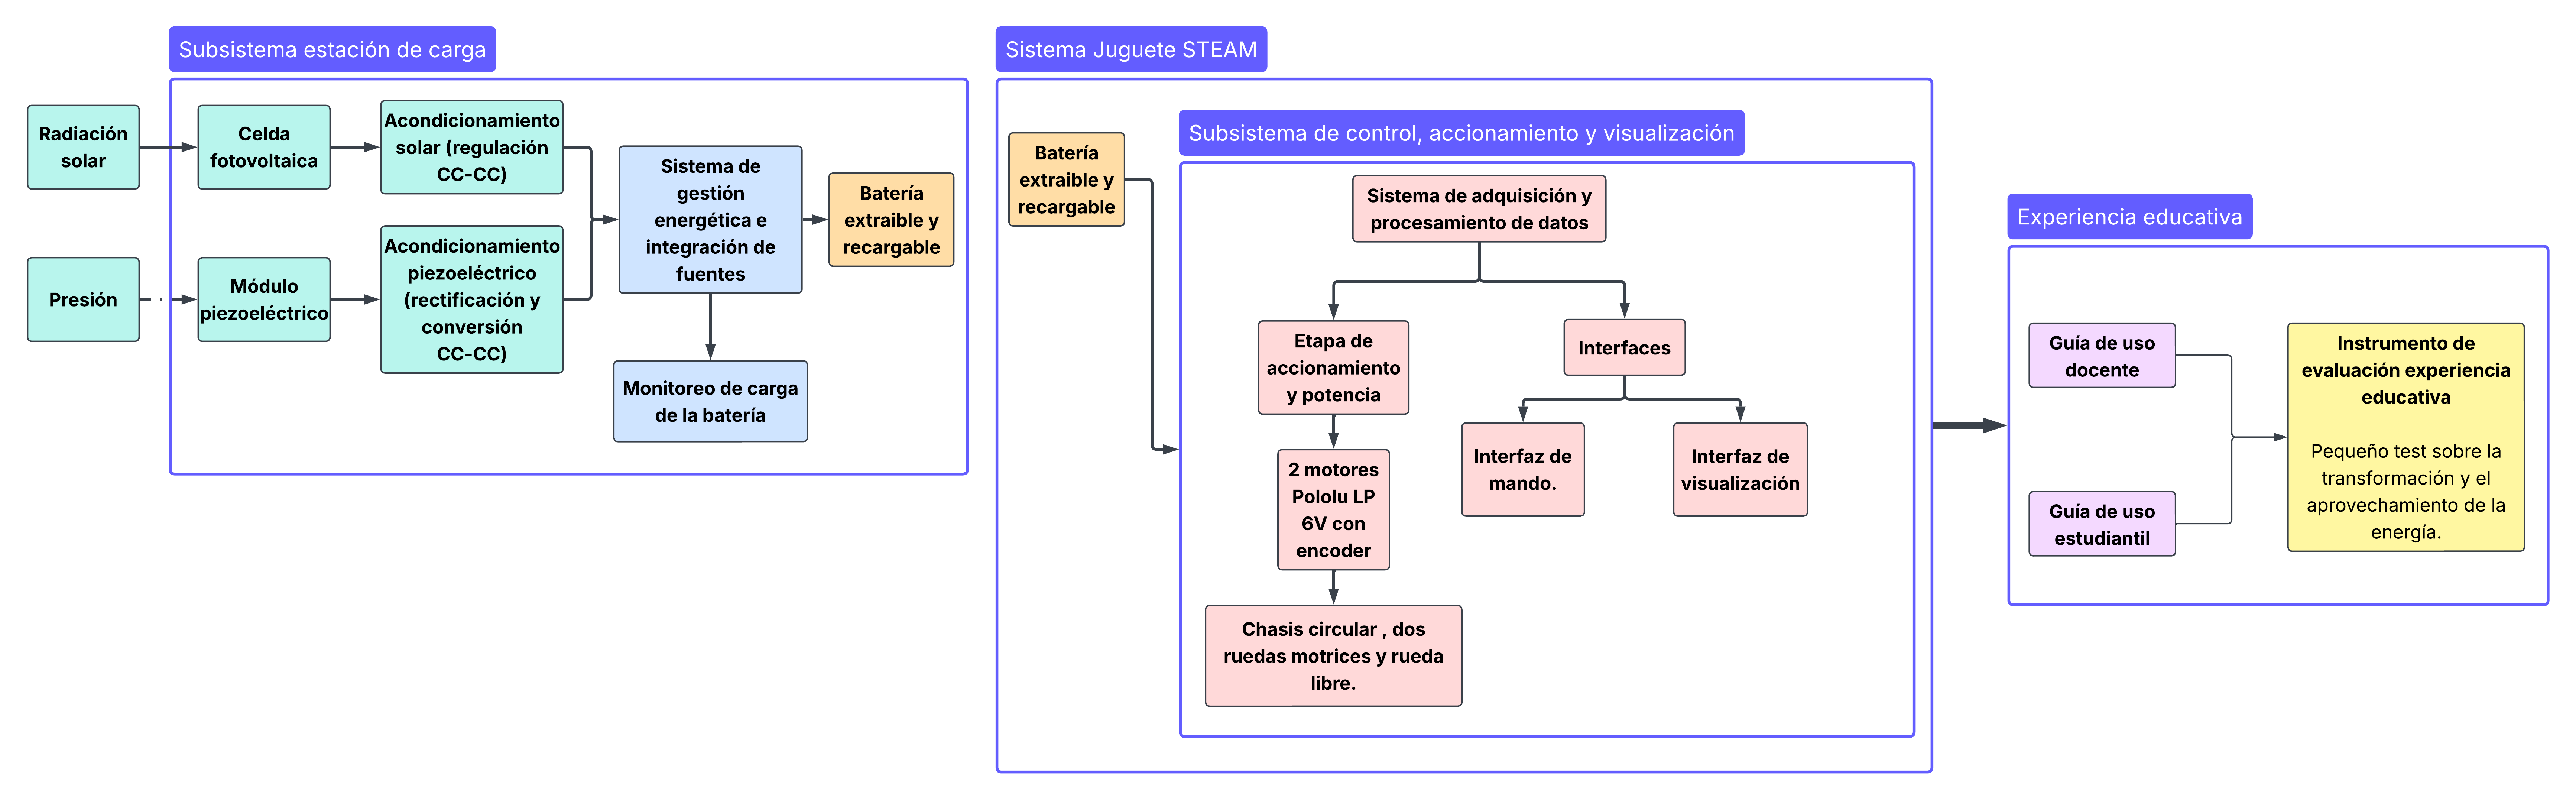
\includegraphics[width=1\columnwidth]{Bloquesfinal.png}
            \caption{Diagrama de bloques Juguete STEAM}
            \label{Fig:bloques}
\end{figure}
\subsection{Estación de carga}

La estación de carga constituye la unidad fija encargada de captar y acondicionar la energía proveniente de las dos fuentes implementadas en el proyecto. Su funcionamiento comprende la conversión de energía solar y mecánica en energía eléctrica, la adaptación de las señales obtenidas y su integración en una etapa de gestión de carga. Esta última permite almacenar la energía en una batería recargable de una celda, que puede retirarse de la estación e instalarse posteriormente en el robot. Adicionalmente, la estación incorpora un mecanismo de monitoreo que permite identificar el estado del proceso de carga.

\subsubsection{Sistema de captación solar}

La energía del panel fotovoltaico se dirige a un cargador solar basado en el
CN3791. Este controlador utiliza una etapa conmutada reductora y realiza el
seguimiento del punto de máxima potencia mediante el pin MPPT y un divisor
resistivo externo. El voltaje objetivo debe configurarse de acuerdo con el
voltaje de máxima potencia especificado para el panel. El fabricante indica
un rango de entrada de \(4.5\) a \(28\,\mathrm{V}\), por lo que el panel y su
punto de operación deben ser compatibles con ese intervalo
\cite{consonance_cn3791_datasheet}.

La corriente de carga se programa mediante una resistencia de sensado y
debe elegirse según la batería y los límites térmicos y
eléctricos de la tarjeta. El valor máximo de \(4\,\mathrm{A}\) especificado
para el controlador no implica que esa sea la corriente adecuada para la
batería \cite{consonance_cn3791_datasheet}.

\subsubsection{Sistema de captación piezoeléctrica}

La segunda fuente corresponde al sistema de captación piezoeléctrica, compuesto por un elemento transductor que convierte la presión mecánica aplicada sobre su superficie en una señal eléctrica. A diferencia de la celda fotovoltaica, cuya salida es de corriente continua, la señal generada por el elemento piezoeléctrico presenta variaciones de amplitud y polaridad asociadas a la aplicación de presión y a la deformación del material.

Por esta razón, la energía obtenida atraviesa una etapa de acondicionamiento piezoeléctrico que comprende la rectificación de la señal y su posterior conversión CC--CC. La rectificación permite obtener una señal de polaridad definida, mientras que la conversión adapta el nivel de tensión para su aprovechamiento en la etapa de gestión energética. De esta manera, se obtiene una salida de corriente continua que puede incorporarse al proceso de almacenamiento energético.

\subsubsection{Integración de fuentes y gestión de carga}

Las salidas de los sistemas fotovoltaico y piezoeléctrico se acondicionan
mediante rutas independientes. La salida fotovoltaica se conecta a un módulo
basado en el controlador CN3791, cuya función es gestionar la carga de la
batería y realizar el seguimiento del punto de máxima potencia (MPPT) del
panel solar. La salida piezoeléctrica requiere rectificación y
acondicionamiento propios; por tanto, no se conecta en paralelo con el panel
a la entrada del CN3791, ya que modificaría las condiciones de operación
utilizadas para el seguimiento del punto de máxima potencia
\cite{consonance_cn3791_datasheet}.

El CN3791 es un controlador conmutado de topología reductora (\textit{buck})
para cargar una batería de ion-litio de una celda. Implementa las etapas de
precarga, corriente constante y tensión constante. En esta última, regula la
tensión de la batería a un valor nominal de \(4.2\,\mathrm{V}\). La corriente
de carga se establece mediante una resistencia externa de sensado, de acuerdo
con las especificaciones de la batería y los límites eléctricos y térmicos
del módulo utilizado \cite{consonance_cn3791_datasheet}.

El seguimiento MPPT del CN3791 utiliza el método de tensión constante: un
divisor resistivo conectado al pin MPPT establece el voltaje de operación
objetivo del panel fotovoltaico. El controlador regula ese punto durante la
carga, siempre que la tensión de entrada se encuentre dentro del rango de
operación especificado, de \(4.5\) a \(28\,\mathrm{V}\). Aunque el circuito
integrado admite una corriente de carga de hasta \(4\,\mathrm{A}\), este
valor máximo no corresponde necesariamente a la corriente apropiada para la
batería del proyecto \cite{consonance_cn3791_datasheet}.

La energía piezoeléctrica se considera una fuente complementaria y
demostrativa. Su incorporación al almacenamiento debe realizarse mediante
una etapa compatible con la salida acondicionada del transductor y con los
requisitos de carga de la batería. En consecuencia, el diagrama del sistema
debe representar por separado la rama fotovoltaica, conectada al cargador
CN3791, y la rama piezoeléctrica, e indicar el punto de integración con la
batería solo cuando se haya definido el circuito correspondiente.

\subsubsection{Monitoreo del estado de carga de la batería}

La estación incorpora un sistema de monitoreo destinado a informar el estado del proceso de carga de la batería. Esta función permite identificar cuándo se está suministrando corriente a la celda y cuándo se ha alcanzado la condición de finalización de carga. Para ello, se aprovechan las salidas de indicación de estado disponibles en el controlador CN3791, las cuales permiten implementar indicadores visuales asociados a las etapas de carga y a su finalización \cite{consonance_cn3791_datasheet}.

Este mecanismo facilita que el estudiante observe la relación entre la disponibilidad de energía en las fuentes de captación y el proceso de almacenamiento en la batería. De esta manera, la estación permite reconocer cuándo se está generando energía aprovechable y cómo esta se transfiere hacia el elemento de almacenamiento.

\subsection{Robot móvil}

El robot móvil corresponde a la unidad encargada de utilizar la energía almacenada en la batería para ejecutar las acciones de movimiento e interacción con el estudiante. Su arquitectura integra una batería extraíble, una unidad de control basada en la tarjeta ESP32-C3 SuperMini, una etapa de accionamiento de motores, dos motores reductores con encoder, una plataforma mecánica y las interfaces de mando y visualización.

\subsubsection{Sistema de alimentación eléctrica}

La alimentación del robot se realiza mediante una batería recargable de ion-litio
o polímero de litio de una celda (1S), con una tensión nominal de
\(3.7\,\mathrm{V}\) y una tensión máxima de carga de \(4.2\,\mathrm{V}\). La
batería se carga en la estación mediante el cargador solar basado en el
controlador CN3791 y, una vez retirada, se instala en el robot. De esta manera,
el mismo elemento de almacenamiento se utiliza en ambas unidades. La corriente
de carga programada debe ajustarse a las especificaciones de la batería y a
los límites del módulo de carga utilizado
\cite{consonance_cn3791_datasheet}.

La alimentación de potencia de los motores sigue la ruta
batería \(\rightarrow\) convertidor elevador \(\rightarrow\) controlador de
motores \(\rightarrow\) motores. Como cada motor tiene una tensión nominal de
\(6\,\mathrm{V}\), se utiliza el convertidor elevador Pololu U3V50F6 para
proporcionar un riel regulado de \(6\,\mathrm{V}\) a la etapa de potencia. Cada
motor recibe \(6\,\mathrm{V}\) nominales a través de un canal independiente
del DRV8833; sus tensiones no se suman para formar una alimentación de
\(12\,\mathrm{V}\). El convertidor admite una tensión de entrada desde
\(2.9\,\mathrm{V}\), por lo que puede operar con una batería de una celda dentro
de las condiciones especificadas por el fabricante
\cite{pololu_u3v50f6}.

La tarjeta ESP32-C3 SuperMini se alimenta mediante una rama regulada separada
del riel de \(6\,\mathrm{V}\) de los motores. La tensión de esa rama y el pin
de alimentación utilizado deben corresponder a la versión específica de la
tarjeta: por ejemplo, una entrada de \(3.3\,\mathrm{V}\) regulados o una
entrada de \(5\,\mathrm{V}\), únicamente si la placa seleccionada la admite.
La salida de \(6\,\mathrm{V}\) destinada a los motores no debe conectarse
directamente a la tarjeta de control. Las tierras de la batería, el
convertidor, el controlador de motores y la tarjeta de control deben compartir
una referencia común.

\subsubsection{Sistema de control y procesamiento}

La unidad de control del robot está constituida por la tarjeta ESP32-C3
SuperMini, que procesa las instrucciones provenientes de la interfaz de mando
y genera las señales necesarias para controlar el movimiento de los motores.
Esta tarjeta integra un microcontrolador de arquitectura RISC-V de 32 bits,
con frecuencia de operación de hasta \(160\,\mathrm{MHz}\), conectividad Wi-Fi
de \(2.4\,\mathrm{GHz}\) y Bluetooth Low Energy (BLE) 5. Además, dispone de
entradas y salidas de propósito general y periféricos de modulación por ancho
de pulso (PWM), utilizados para generar las señales de control de los
actuadores \cite{espressif_esp32c3}.

El microcontrolador recibe las instrucciones de movimiento, determina el
sentido de giro y genera las señales de dirección y PWM que envía a las
entradas lógicas del controlador DRV8833. Este controlador utiliza dichas
señales para regular el sentido de giro y la velocidad de cada motor. Asimismo,
la ESP32-C3 recibe las señales procedentes de los encoders instalados en los
motores y registra los pulsos asociados al desplazamiento de las ruedas. Esta
información puede utilizarse para estimar la velocidad de giro y realizar
ajustes en el accionamiento de cada motor.

\subsubsection{Etapa de accionamiento y potencia}

La etapa de accionamiento está conformada por un controlador de motores
DRV8833, implementado mediante la tarjeta Pololu DRV8833 Dual Motor Driver
Carrier. Este dispositivo integra dos puentes H independientes y permite
controlar dos motores de corriente continua con escobillas, regulando
individualmente su sentido de giro y velocidad \cite{pololu_drv8833,ti_drv8833}.

La tarjeta se alimenta desde el riel regulado de \(6\,\mathrm{V}\) y cada uno
de sus canales acciona un motor Pololu LP de \(6\,\mathrm{V}\). Por tanto, cada
motor opera con su tensión nominal de \(6\,\mathrm{V}\); las tensiones de los
dos motores no se suman para establecer una alimentación de \(12\,\mathrm{V}\).
De acuerdo con las especificaciones del fabricante, esta familia presenta una
corriente típica en vacío de aproximadamente \(40\,\mathrm{mA}\) y una corriente
de bloqueo de \(360\,\mathrm{mA}\) por motor a su tensión nominal de
\(6\,\mathrm{V}\) \cite{pololu_lp_6v}. Si ambos motores alcanzaran
simultáneamente la condición de bloqueo, la corriente total sería
aproximadamente \(720\,\mathrm{mA}\).

La tarjeta DRV8833 seleccionada permite entregar una corriente continua de
hasta \(1.2\,\mathrm{A}\) por canal y una corriente pico de \(2\,\mathrm{A}\)
por canal, con un intervalo de alimentación de motores comprendido entre
\(2.7\,\mathrm{V}\) y \(10.8\,\mathrm{V}\) \cite{pololu_drv8833}. Estos valores
corresponden a los límites especificados para la tarjeta; la corriente
disponible en la aplicación también depende de la disipación térmica y de las
condiciones de operación.

La ESP32-C3 envía las señales de dirección y PWM a las entradas lógicas del
DRV8833. El controlador conmuta la alimentación del riel de potencia para
entregar a cada motor la corriente que requiere. Así, los pines de la
ESP32-C3 se utilizan para transmitir señales de control y no para alimentar
directamente los motores.

\subsubsection{Actuadores y sistema mecánico}

El movimiento del juguete se genera mediante dos motores reductores DC Pololu LP de 6 V, cada uno equipado con un encoder incremental. Los motores se encargan de proporcionar el par necesario para accionar las ruedas motrices, mientras que los encoders generan señales de realimentación que permiten registrar el giro de cada eje. La información obtenida se transmite hacia la unidad de control, donde se procesa para determinar el comportamiento de los motores durante el desplazamiento.

La plataforma mecánica está conformada por un chasis circular, dos ruedas motrices acopladas a los motores y una rueda libre que proporciona un punto adicional de apoyo. Esta configuración corresponde a un sistema de tracción diferencial, en el cual el desplazamiento y la orientación del robot se determinan mediante la regulación independiente de la velocidad y el sentido de giro de las dos ruedas motrices. Así, el control coordinado de ambos motores permite ejecutar desplazamientos hacia adelante, hacia atrás y realizar giros sobre la superficie de operación.

\subsubsection{Interfaces de interacción y visualización}

La interacción con el robot se realiza mediante una interfaz de mando que permite al estudiante enviar instrucciones de movimiento a la unidad de control. Esta comunicación se establece mediante Bluetooth Low Energy, aprovechando la conectividad integrada en la ESP32-C3 SuperMini. De esta manera, las instrucciones enviadas desde un dispositivo externo son recibidas y procesadas por el microcontrolador para controlar el desplazamiento del juguete.

Adicionalmente, se incorpora una interfaz de visualización mediante una pantalla OLED, destinada a presentar información relacionada con el funcionamiento del robot. Esta interfaz permite comunicar al usuario estados de operación y datos relevantes para el desarrollo de las actividades educativas. La integración de ambos elementos facilita la interacción directa con el prototipo y permite relacionar las instrucciones del estudiante con la respuesta física del sistema.

\subsection{Experiencia educativa}

La experiencia educativa se desarrolla mediante el uso conjunto de la estación de carga y el robot móvil, acompañados por una guía de uso docente y una guía de uso estudiantil. La guía docente establece las orientaciones para la preparación y ejecución de las actividades, mientras que la guía estudiantil presenta las instrucciones necesarias para interactuar con las fuentes de captación, observar el proceso de almacenamiento y utilizar la batería en el robot.

Durante la actividad, los estudiantes pueden observar cómo la radiación solar y la presión mecánica son transformadas en energía eléctrica, cómo esta energía es acondicionada y almacenada en una batería y cómo posteriormente se utiliza para alimentar el movimiento del juguete. El intercambio de la batería entre la estación y el robot permite relacionar los procesos de adquisición y consumo energético dentro de una misma experiencia práctica.

Finalmente, se incorpora un instrumento de evaluación compuesto por preguntas orientadas a analizar la comprensión de los estudiantes sobre las fuentes de energía utilizadas, los procesos de transformación, el almacenamiento energético y el aprovechamiento de la energía eléctrica en el funcionamiento del robot. Este instrumento permite valorar el aporte de la experiencia a la comprensión de los conceptos abordados.

\subsection{Evaluación de la solución}

La evaluación de la solución comprende pruebas independientes para la estación de carga, el robot móvil y la integración de ambos sistemas, además de la aplicación del instrumento de evaluación educativa. En la estación se realizarán pruebas de generación fotovoltaica bajo diferentes condiciones de iluminación y pruebas de generación piezoeléctrica mediante la aplicación de presión sobre el transductor. En ambos casos se registrarán las variables eléctricas de salida para determinar la potencia entregada, considerando la relación entre tensión y corriente, y estimar la energía obtenida durante los intervalos de operación.

También se verificará el acondicionamiento de las fuentes y el funcionamiento del módulo CN3791 durante el proceso de carga. Para ello, se registrarán la tensión de la batería, la corriente de carga y los indicadores de estado, con el propósito de comprobar la transferencia de energía y la finalización del proceso de almacenamiento.

En el robot móvil se realizarán pruebas de accionamiento individual y simultáneo de los motores, verificando el sentido de giro, la respuesta ante diferentes señales PWM y el comportamiento de los encoders. Adicionalmente, se evaluará el desplazamiento sobre una superficie de prueba, los giros de la plataforma, la estabilidad mecánica y el consumo eléctrico durante la operación. Estas pruebas permitirán comprobar que la etapa de potencia y el sistema de control responden adecuadamente a las instrucciones suministradas por el estudiante.

Finalmente, se realizarán pruebas de integración mediante el intercambio de la batería entre la estación y el robot, verificando el funcionamiento conjunto de los sistemas de captación, acondicionamiento, almacenamiento, control y actuación. Se analizará la energía obtenida en la estación y el consumo registrado durante el funcionamiento del juguete, con el fin de caracterizar el aporte de los sistemas de Energy Harvesting a la alimentación del prototipo. La evaluación educativa se complementará con la aplicación del instrumento diseñado para analizar la comprensión de los conceptos relacionados con la transformación y el aprovechamiento de la energía.

% ================= planeacion_trabajo =================
\newpage
\section{Planeación del Trabajo}
El proyecto se desarrollará en cinco fases principales. Inicialmente, se llevará a cabo el diseño y construcción mecánica del prototipo, seguido del diseño e implementación de los componentes electrónicos. Posteriormente, se realizará el desarrollo del software necesario para el funcionamiento y control del sistema. Una vez completados estos componentes, se procederá con la integración de los subsistemas, las pruebas de funcionamiento y la validación del prototipo. Finalmente, se realizará la documentación de los resultados y la preparación de los entregables y la presentación final del proyecto. Estas fases permiten organizar el alcance del trabajo de manera secuencial y establecer una base para la planificación de las actividades mediante los diagramas WBS y Gantt.

\begin{figure}[H]
            \centering
            \includegraphics[width=0.9\columnwidth]{WBSjug.png}
            \caption{Diagrama WBS Diseño de un juguete STEAM}
            \label{Fig:WBS}
\end{figure}

\begin{figure}[H]
            \centering
            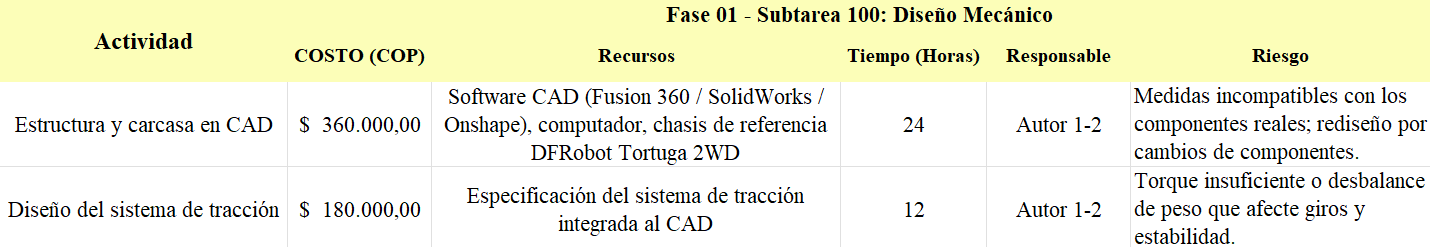
\includegraphics[width=0.9\columnwidth]{fase 1-100.png}
            \caption{Cuadro de detalles de las actividades subtarea 1 (01-01-100)
}
            \label{Fig:fase1-100}
\end{figure}


\begin{figure}[H]
            \centering
            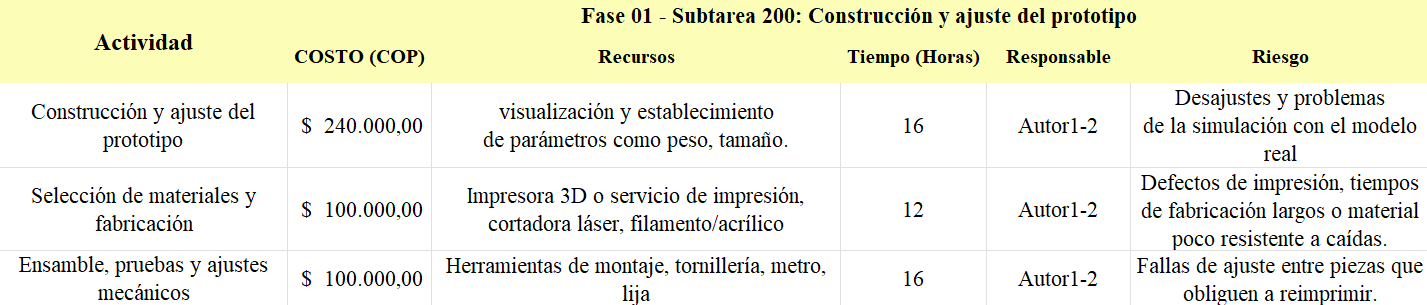
\includegraphics[width=0.9\columnwidth]{fase 1-200.png}
            \caption{Cuadro de detalles de las actividades subtarea 1 (01-01-200)
}
            \label{Fig:fase1-200}
\end{figure}


\begin{figure}[H]
            \centering
            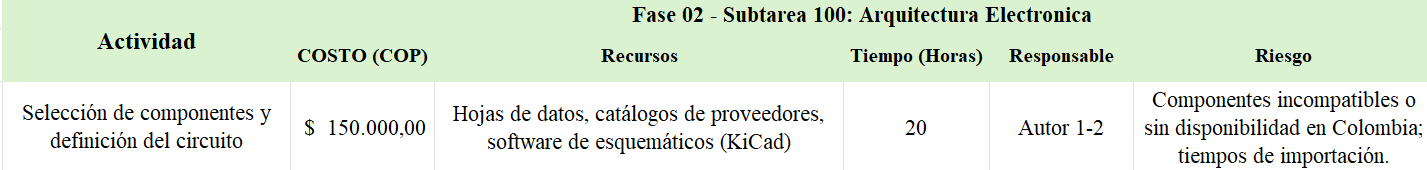
\includegraphics[width=0.9\columnwidth]{fase 2-100.png}
            \caption{Cuadro de detalles de las actividades subtarea 2 (01-02-100)
}
            \label{Fig:fase 2-100}
\end{figure}

\begin{figure}[H]
            \centering
            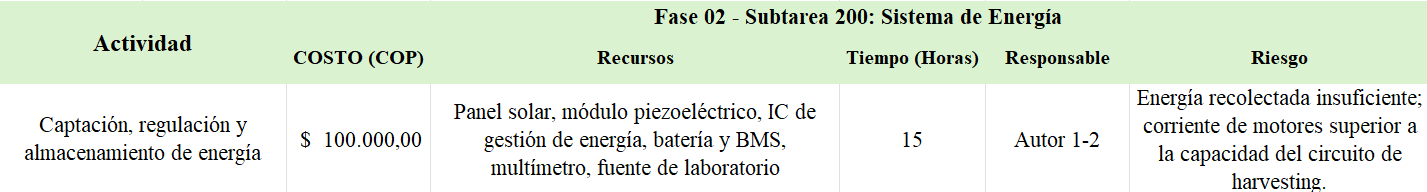
\includegraphics[width=0.9\columnwidth]{fase 2-200.png}
            \caption{Cuadro de detalles de las actividades subtarea 2 (01-02-200)
}
            \label{Fig:fase2-200}
\end{figure}

\begin{figure}[H]
            \centering
            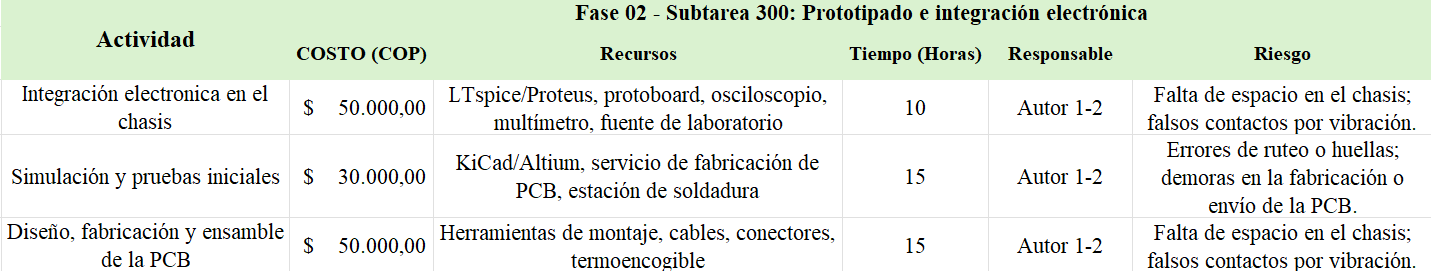
\includegraphics[width=0.9\columnwidth]{fase 2-300.png}
            \caption{Cuadro de detalles de las actividades subtarea 2 (01-02-300)}
            \label{Fig:fase 2-300}
\end{figure}

\begin{figure}[H]
            \centering
            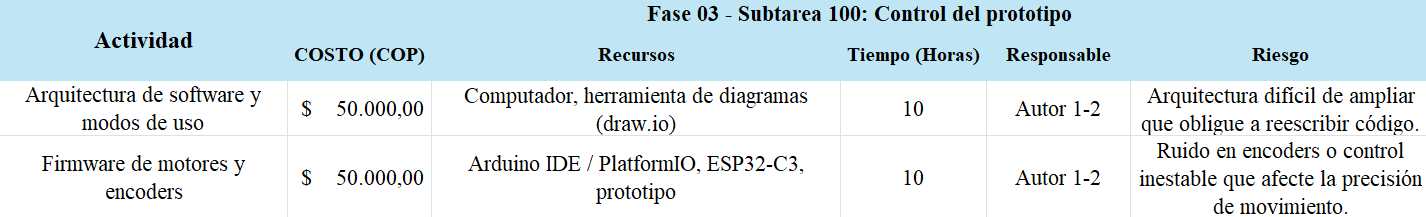
\includegraphics[width=0.9\columnwidth]{fase 3-100.png}
            \caption{Cuadro de detalles de las actividades subtarea 3 (01-03-100)}
            \label{Fig:fase 3-100}
\end{figure}

\begin{figure}[H]
            \centering
            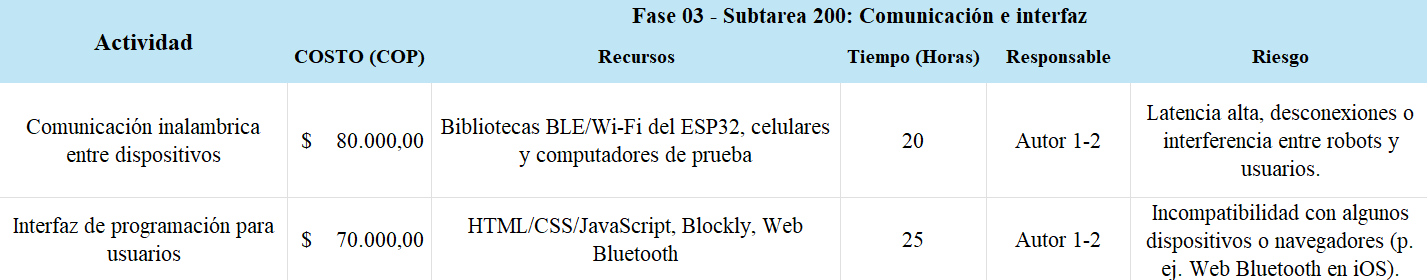
\includegraphics[width=0.9\columnwidth]{fase 3-200.png}
            \caption{Cuadro de detalles de las actividades subtarea 3 (01-03-200)}
            \label{Fig:fase 3-200}
\end{figure}

\begin{figure}[H]
            \centering
            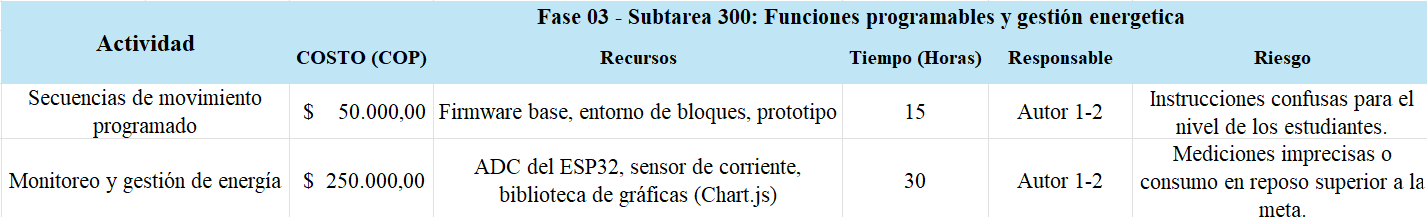
\includegraphics[width=0.9\columnwidth]{fase 3-300.png}
            \caption{Cuadro de detalles de las actividades subtarea 3 (01-03-300)}
            \label{Fig:fase 3-300}
\end{figure}

\begin{figure}[H]
            \centering
            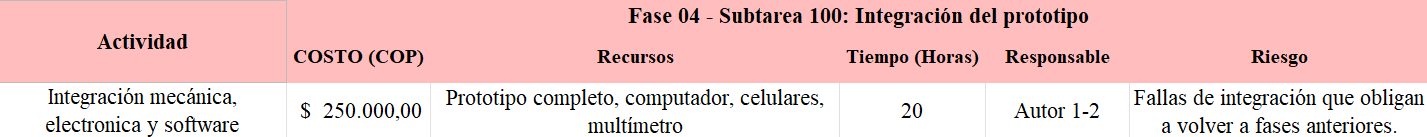
\includegraphics[width=0.9\columnwidth]{fase 4-100.png}
            \caption{Cuadro de detalles de las actividades subtarea 4 (01-04-100)}
            \label{Fig:fase 4-100}
\end{figure}

\begin{figure}[H]
            \centering
            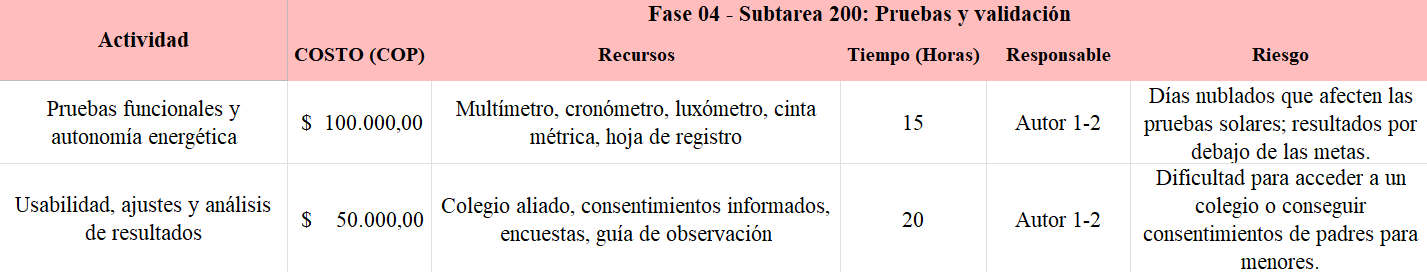
\includegraphics[width=0.9\columnwidth]{fase 4-200.png}
            \caption{Cuadro de detalles de las actividades subtarea 4 (01-04-200)}
            \label{Fig:fase 4-200}
\end{figure}

\begin{figure}[H]
            \centering
            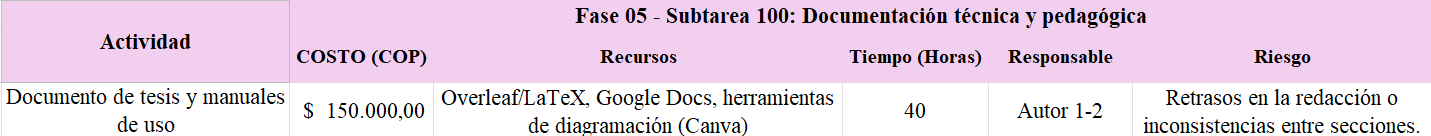
\includegraphics[width=0.9\columnwidth]{fase 5-100.png}
            \caption{Cuadro de detalles de las actividades subtarea 5 (01-05-100)}
            \label{Fig:fase 5-100}
\end{figure}

\begin{figure}[H]
            \centering
            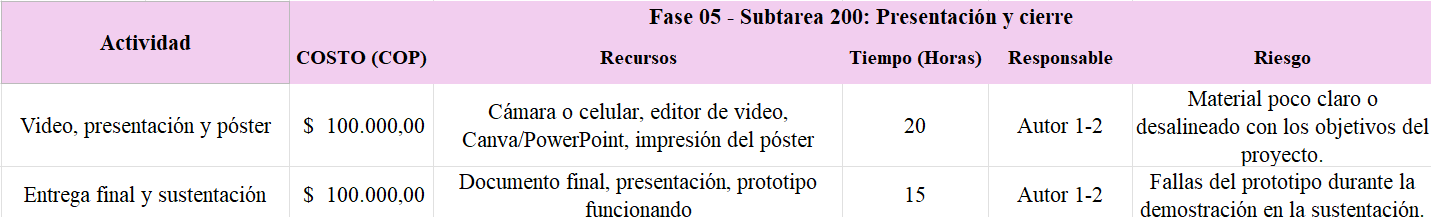
\includegraphics[width=0.9\columnwidth]{fase 5-200.png}
            \caption{Cuadro de detalles de las actividades subtarea 5 (01-05-200)}
            \label{Fig:fase 5-200}
\end{figure}

 
\subsection{Diagrama de Gantt}


La figura \ref{gantt_1} corresponde al diagrama de Gantt previsto para el desarrollo del Juguete STEAM.

\begin{figure}[H]
            \centering
            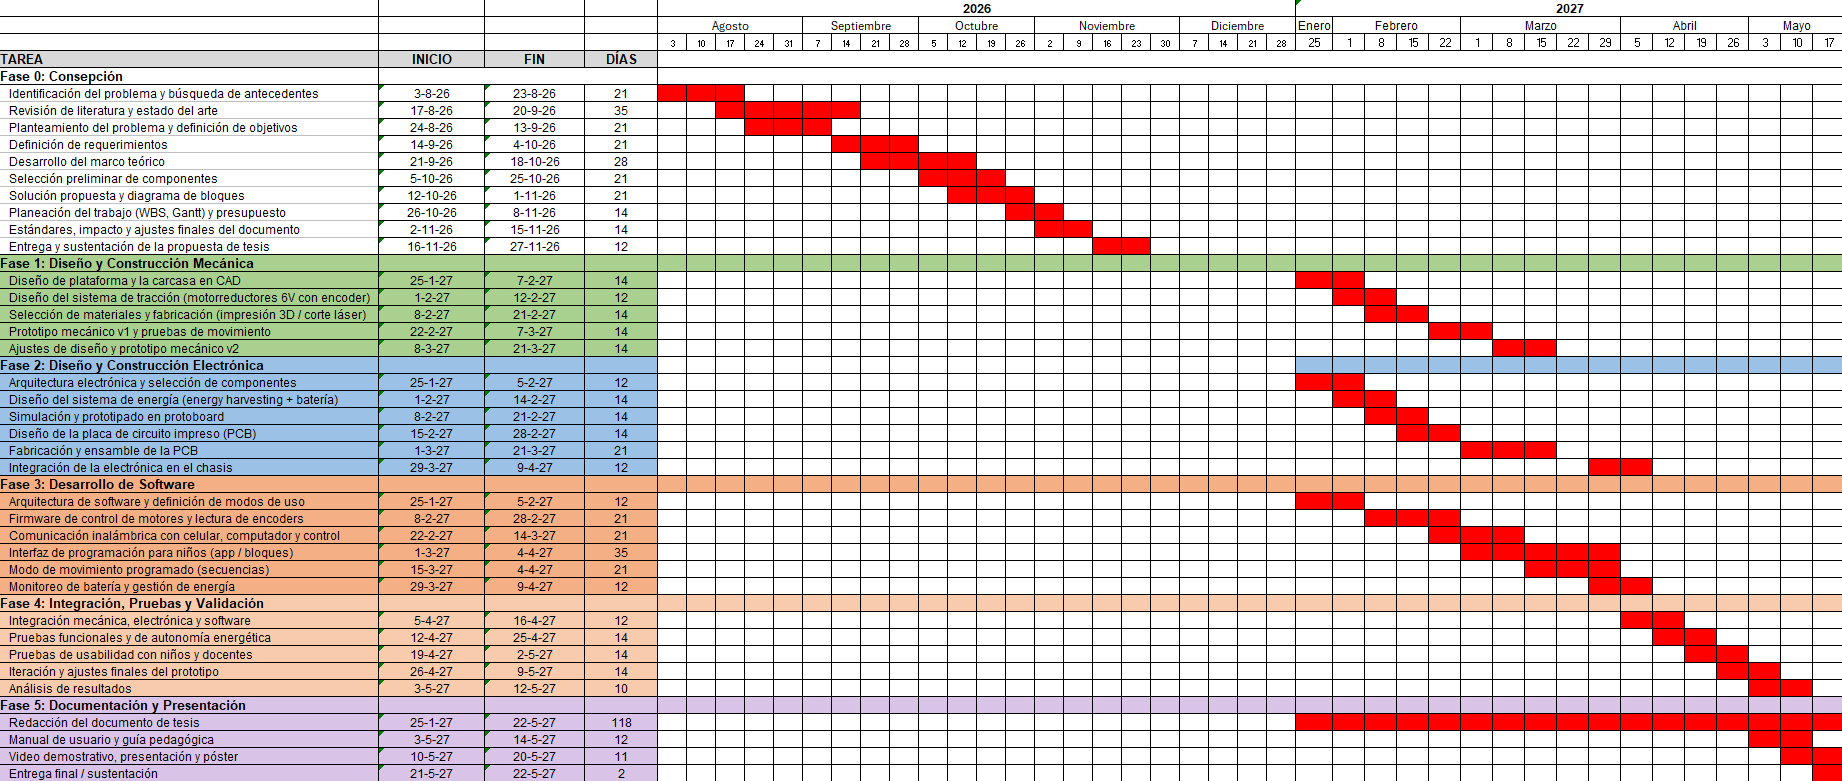
\includegraphics[width=1\columnwidth]{Diagrama de gantt.png}
            \caption{Ejemplo de Diagrama de Gantt juguete STEAM}
            \label{gantt_1}
\end{figure}

% ================= presupuesto =================
\newpage
\section{Presupuesto}
El presupuesto estimado para el desarrollo del proyecto se presenta en la Tabla 4, organizado en cinco rubros: recursos humanos, materiales, equipos, software y otros servicios. Para cada ítem se indica la cantidad, el costo unitario en pesos colombianos (COP), el tiempo de uso y la fuente de financiación, ya sea propia (los autores) o de la Pontificia Universidad Javeriana (PUJ). Excluyendo las horas de trabajo, el subtotal de los rubros cuantificados asciende a \$8.069.939 COP. A este valor se suman las horas de trabajo de los autores y del director, los costos de envío e impuestos y un 10 \% de imprevistos, para un total estimado de \$[8.069.939,00] COP.

El rubro de recursos humanos corresponde a las horas de trabajo del director y de los dos autores durante las [N] semanas del proyecto, de acuerdo con la planeación de la Figura 3. Se estiman [X] horas por autor y [Y] horas de asesoría del director, valoradas en \$[valor/hora] COP, para un total de \$[valor] COP. Las horas de los autores se asumen como financiación propia, y las del director, como aporte de la PUJ.

Los materiales, por un valor de \$314.000 COP, corresponden a los componentes necesarios para construir los subsistemas definidos en la solución propuesta. El sistema de energy harvesting está compuesto por cuatro transductores piezoeléctricos, dos paneles solares y un conversor de alimentación encargado de acondicionar la energía recolectada. La energía se almacena en dos baterías de litio con su respectivo cargador. Esta configuración permite operar el juguete cuando la energía recolectada es insuficiente, condición que la literatura reporta como habitual en plataformas móviles alimentadas por fuentes ambientales pequeñas. El sistema de control se basa en un ESP32-C3 Super Mini, que gestiona los motores y la comunicación inalámbrica. La actuación e interacción se completan con dos elementos de tracción y una pantalla OLED, que permite al estudiante visualizar variables del sistema energético. Se incluye además un rubro de componentes electrónicos menores para resistencias, condensadores, conectores y cableado. Se priorizaron componentes comerciales de bajo costo y fácil adquisición en el mercado local, de modo que el prototipo pueda reproducirse y repararse con facilidad, lo cual es coherente con su uso en instituciones educativas.

Los equipos de laboratorio (fuente de alimentación, osciloscopio, multímetro, generador de señales y estación de soldadura) suman \$4.545.939 COP. Son indispensables para caracterizar la capacidad de generación de los harvesters, verificar el funcionamiento de las etapas de acondicionamiento y ensamblar la PCB. Su uso se estima durante seis meses y la PUJ los aporta a través de sus laboratorios. Del mismo modo, las licencias de Altium Designer (\$1.200.000 COP, dos meses) y SolidWorks (\$1.700.000 COP, un mes) se requieren para el diseño de la PCB y el modelado CAD del chasis, respectivamente, y también las aporta la universidad.

En el rubro de otros servicios se contemplan la fabricación del circuito impreso (\$60.000 COP), la impresión y el corte del chasis (\$100.000 COP) y cinco visitas de campo (\$150.000 COP). Estas últimas son necesarias para aplicar la experiencia educativa con estudiantes de bachillerato y evaluar el cuarto objetivo específico.

En cuanto a la distribución de la financiación, la PUJ asume \$7.445.939 COP en equipos y licencias, que corresponde al 92 \% del subtotal cuantificado, y los autores asumen \$624.000 COP en materiales y servicios. Esto evidencia que el costo directo del prototipo es bajo y que la mayor parte de la inversión corresponde a infraestructura ya disponible en la universidad. Esta condición favorece la viabilidad del proyecto y la posibilidad de replicar el juguete en otros contextos educativos.

En el presupuesto se sugiere cuantificar los diferentes rubros, los cuales \textbf{pueden} ser divididos en: 

\begin{itemize}
    \item Recursos Humanos
    \item Materiales
    \item Equipos
    \item Software
    \item Transporte 
    \item Otros (Servicios de alquiler, servicios de impresión, servicios de fabricación, etc.)

\end{itemize}

\begin{figure}[H]
            \centering
            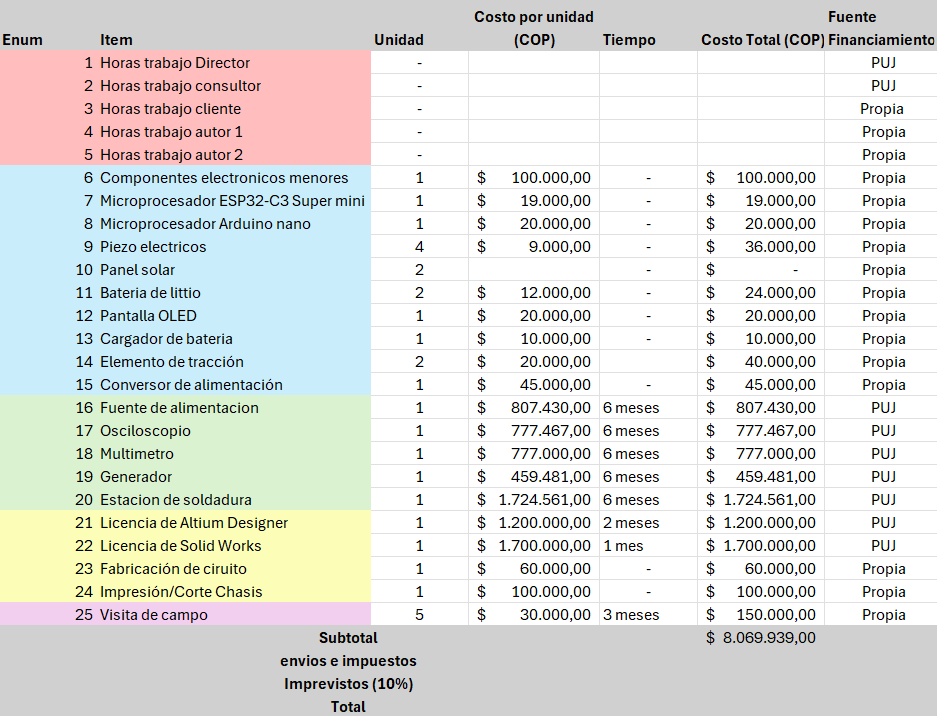
\includegraphics[width=1\columnwidth]{Tabla de costos1.png}
            \caption{Presupuesto del proyecto}
            \label{fig:tabla_costos}
\end{figure}


\vspace{12pt}\par



% ================= estandares =================
\newpage

\section{Estándares aplicados en el proyecto}
Para el desarrollo del juguete STEAM se consideran normas técnicas, reglamentos y protocolos relacionados con la seguridad de los juguetes, la integración de componentes electrónicos, el almacenamiento energético, la comunicación inalámbrica y el diseño de interfaces. Asimismo, se tienen en cuenta referentes curriculares nacionales para orientar las actividades educativas dirigidas a estudiantes de bachillerato. En la Tabla~\ref{tab:estandares} se presentan los principales estándares y su aplicación en los componentes y actividades del proyecto.

\begin{table}[H]
\centering
\renewcommand{\arraystretch}{1.2}

\begin{tabular}{|p{3.5cm}|p{5cm}|p{7cm}|}
\hline
\textbf{Estándar} &
\textbf{Descripción breve} &
\textbf{Aplicación en el proyecto} \\
\hline

Resolución 686 de 2018 y Resolución 407 de 2024 &
Reglamento técnico colombiano relacionado con los requisitos de seguridad y evaluación de conformidad de juguetes. &
Se consideran como referencia para el diseño seguro de la estación de carga y el robot móvil, teniendo en cuenta sus componentes eléctricos, mecánicos y las condiciones de utilización del prototipo. \\
\hline

ISO 8124-1 e ISO 8124-2 &
Establecen requisitos de seguridad mecánica y física, así como criterios de inflamabilidad para juguetes. &
Se toman como referencia para el diseño del chasis, las ruedas, los mecanismos móviles y las piezas fabricadas en PLA, buscando reducir riesgos asociados a bordes y partes móviles. \\
\hline

IEC 62115:2017 &
Establece requisitos de seguridad para juguetes eléctricos. &
Se considera para la integración eléctrica de la estación de carga y el robot, especialmente en las conexiones, los motores, el controlador, la batería y los circuitos de alimentación. \\
\hline

IEC 62133-2:2017 &
Define requisitos y ensayos de seguridad para celdas y baterías recargables de litio. &
Se considera para la utilización de la batería recargable de una celda, teniendo en cuenta los riesgos de cortocircuito, sobrecalentamiento, daño mecánico y condiciones de carga. \\
\hline

Bluetooth Core Specification 5.0 &
Define las especificaciones técnicas para la comunicación inalámbrica Bluetooth, incluyendo Bluetooth Low Energy (BLE). &
Se aplica a la comunicación entre la interfaz de mando y la tarjeta ESP32-C3 SuperMini, permitiendo transmitir las instrucciones para controlar el desplazamiento del robot. \\
\hline

ISO 9241-210:2019 &
Proporciona principios para el diseño centrado en las personas de sistemas interactivos. &
Se considera para el diseño de las interfaces de mando y visualización, buscando que la interacción con el robot y la información presentada en la pantalla OLED sean comprensibles para los estudiantes. \\
\hline

Guía 30 y Orientaciones Curriculares de Tecnología e Informática del MEN &
Proporcionan referentes para el desarrollo de competencias tecnológicas y científicas en la educación básica y media. &
Se utilizan como referencia para estructurar las guías docente y estudiantil y el instrumento de evaluación, relacionando las actividades con la transformación y el aprovechamiento de la energía. \\
\hline

\end{tabular}

\caption{Estándares aplicados en el proyecto}
\label{tab:estandares}
\end{table}

\noindent\footnotesize
\textit{Nota: Las normas de seguridad de juguetes citadas contemplan productos destinados a menores de 14 años. Dado que la experiencia educativa se dirige a estudiantes de grados noveno a once, se consideran como referencias de diseño seguro; su aplicabilidad reglamentaria dependerá de la clasificación por edad del producto y de las condiciones de fabricación y comercialización. Su inclusión no constituye una declaración de certificación o conformidad del prototipo.}
\normalsize


% ================= impacto =================
\newpage
\section{Impacto Socio-económico y ambiental}
El desarrollo de este proyecto puede generar impactos positivos en el ámbito social al proporcionar una herramienta didáctica interactiva para estudiantes de bachillerato, particularmente de los grados noveno a once, que facilite la comprensión de conceptos relacionados con la generación, transformación, almacenamiento y aprovechamiento de la energía. Mediante la interacción con el juguete, los estudiantes podrán observar cómo la energía solar y la energía mecánica asociada al efecto piezoeléctrico se convierten en energía eléctrica y cómo esta puede acondicionarse y almacenarse para alimentar los sistemas del prototipo. De esta manera, se busca complementar la enseñanza teórica mediante experiencias de experimentación que relacionen los conocimientos de ciencia, tecnología, ingeniería, artes y matemáticas. Este enfoque coincide con investigaciones que han identificado resultados favorables en el aprendizaje, la creatividad y la participación estudiantil mediante actividades prácticas STEAM \cite{kanapathy2024,hsiao2022}. Asimismo, el juguete podría constituir un recurso de apoyo para docentes e instituciones educativas interesadas en desarrollar actividades relacionadas con la educación energética. Sin embargo, su aprovechamiento dependerá de la disponibilidad del dispositivo, de la capacitación necesaria para utilizarlo y de la existencia de guías que orienten las actividades, ya que la complejidad de sus componentes electrónicos podría dificultar su implementación sin acompañamiento.

Por otro lado, desde el punto de vista económico, el proyecto contempla la fabricación de un prototipo mediante materiales de impresión 3D y componentes electrónicos comerciales, lo que permite explorar una alternativa de desarrollo local y facilita la posibilidad de realizar modificaciones, reparaciones y ajustes durante su construcción. Además, la integración de los sistemas de captación y almacenamiento energético en un mismo dispositivo puede servir como referencia para futuros desarrollos educativos relacionados con la mecatrónica y las energías renovables. No obstante, la fabricación requiere una inversión inicial en elementos como el panel fotovoltaico, los transductores piezoeléctricos, el circuito de gestión energética, la batería, los actuadores y los sistemas de control, a lo que se suman los costos de impresión, ensamblaje y mantenimiento. Por consiguiente, aunque el diseño puede facilitar la reproducción del prototipo utilizando herramientas de fabricación disponibles, no se puede asegurar una reducción de costos frente a otras alternativas sin realizar una comparación económica. De igual forma, la cantidad de energía recolectada dependerá de las condiciones de iluminación y de la excitación mecánica, por lo que el sistema de Energy Harvesting se plantea como un aporte complementario al almacenamiento energético y no como garantía de alimentación autónoma y continua de todos el sistema.

En el ámbito ambiental, la incorporación de tecnologías solar y piezoeléctrica representa una oportunidad para demostrar experimentalmente el aprovechamiento de fuentes energéticas disponibles en el entorno y promover en los estudiantes una mayor comprensión de las alternativas de generación eléctrica. Adicionalmente, el sistema permitirá abordar el papel del almacenamiento energético y la utilización de la energía recolectada en aplicaciones tecnológicas de pequeña escala. Sin embargo, estos beneficios deben analizarse considerando que el prototipo también requiere materiales de fabricación, circuitos electrónicos y una batería de litio, cuyos procesos de producción y disposición final pueden generar residuos e impactos ambientales. Particularmente, la utilización de componentes electrónicos y baterías exige considerar su mantenimiento, reutilización y gestión adecuada al finalizar su vida útil, mientras que el uso de PLA en las piezas impresas no elimina la necesidad de controlar el consumo de material y los residuos generados durante la fabricación. En este sentido, el aporte ambiental del proyecto no radica en afirmar que el juguete sustituye fuentes convencionales de electricidad, sino en aprovechar parcialmente la energía disponible y utilizar su funcionamiento como medio para enseñar principios de eficiencia, transformación y aprovechamiento energético. Así, el impacto esperado integra la formación científica de los estudiantes, las posibilidades de fabricación y reproducción del dispositivo y la sensibilización frente al uso responsable de los recursos energéticos y materiales.

% ================= declaracion =================
\newpage
\section{Declaración de Uso de Inteligencia Artificial}

Durante el desarrollo del presente trabajo de grado se utilizaron herramientas de inteligencia artificial como apoyo complementario en actividades de revisión y organización del documento, para esta tarea se utilizó Chat GPT. Su utilización se limitó principalmente a la corrección de estilo y redacción, la identificación de posibles inconsistencias en la estructura del texto y la elaboración de listas de verificación (checklists) para identificar apartados, elementos o requisitos pendientes de completar. Adicionalmente, estas herramientas se emplearon como apoyo para mejorar la claridad de algunas explicaciones técnicas, revisar la coherencia entre secciones y facilitar la organización de la información presentada.

Por otro lado la inteligencia artificial Claud para la comparación de componentes y detalles y especificaciones de estos, finalmente se utilizo la IA de Leapspace para agilizar y filtración procesos de busqueda de información y articulos scientificos para la debida documentación de respaldo

El uso de estas herramientas no reemplazó el proceso de investigación, diseño, análisis, desarrollo ni toma de decisiones del proyecto. La selección de componentes, el planteamiento de la solución, el desarrollo técnico y la interpretación de los resultados fueron realizados por los autores. Asimismo, las sugerencias generadas mediante inteligencia artificial fueron revisadas y evaluadas antes de su incorporación al documento, siendo los autores responsable del contenido final presentado.


% Referencias
% ================= referencias =================
% ============================================================
%  REFERENCIAS
%  INSTRUCCIONES — no aparecen en el PDF compilado
%
%  - Formato IEEE estrictamente. Orden por aparición en el texto, no alfabéticamente.
%  - Toda referencia debe tener URL (enlace al documento) o DOI.
%  - Toda referencia listada debe estar citada en el texto.
%  - Referencias incompletas (sin año, sin revista, sin DOI) no son válidas.
%  - Más del 50% de referencias con más de 5 años es observación crítica.
%  - Revise duplicados
% ============================================================
\newpage
\nocite{*}

% Tamaño de letra SOLO para la bibliografía (no afecta al resto del documento)
\begingroup
\renewcommand*{\bibfont}{\fontsize{8}{10}\selectfont}
\printbibliography
\endgroup
\addcontentsline{toc}{section}{Referencias}


% Apéndices
% ================= apendice_a =================
\newpage
\section{Anexos}
Incluya en esta sección únicamente los documentos que \textbf{respalden o complementen} el contenido del documento, pero que por su extensión o naturaleza no deben ir en el cuerpo principal. 

\par \vspace{12pt}

Ejemplos: consentimientos informados, protocolos de prueba, inventarios, hojas de datos técnicos, etc.
\par \vspace{12pt}

Cada anexo debe estar identificado con una letra (Anexo A, Anexo B…) y un título descriptivo, y debe ser \textbf{referenciado explícitamente} en el texto del documento.

\subsection{Este sería un subtítulo del anexo A}


\end{document}
